\documentclass[a4paper,10pt]{article}
\usepackage[utf8]{inputenc}
\usepackage[margin=1.5cm, bottom=2cm]{geometry}
\usepackage{fancyhdr}
\usepackage{enumitem}
\usepackage{xcolor}
\usepackage[most]{tcolorbox}
\newtcolorbox{osservazioni}{
  colback=gray!8,    % sfondo grigio chiaro
  colframe=white,      % nessun bordo
  arc=2mm,            % angoli smussati
  boxrule=0pt,        % spessore bordo 0
  fontupper=\footnotesize,
  left=2mm, right=2mm, top=2mm, bottom=2mm,
  before skip=7pt,   % niente spazio prima
  after skip=15pt     % niente spazio dopo
}
\pagestyle{fancy}
\usepackage{tikz}
\usetikzlibrary{automata, positioning}
\pagestyle{fancy}


%%%%%%%%%%%%%%%%%%%
\newcommand{\EsercitazioneNum}{06}
\newcommand{\Data}{21/09/2025}
%%%%%%%%%%%%%%%%%%%

% Numero di pagina in basso al centro
\fancyhf{}
\fancyfoot[C] \thepage
\renewcommand{\footrulewidth}{0pt} % niente linea in basso
\renewcommand{\headrulewidth}{0pt} % niente linea in alto

\begin{document}
\footnotesize  % font generale più piccolo

\noindent
\small \textbf{Computabilità, Complessità e Logica - a.a. 2025/26} \hfill \textbf{Esercitazione \EsercitazioneNum} \\[0.2cm]
\scriptsize Matteo Liotta, \texttt{matteo.liotta@studenti.units.it} \hfill \Data \\[0.2cm]

\noindent\makebox[\linewidth]{\rule{\linewidth}{0.4pt}} \\[1cm]


\noindent\Large \addcontentsline{toc}{Esercitazione 06: \textit{Automi a Pila e Grammatiche Libere dal contesto}}{section} \textbf{Esercitazione 06}: \textit{Automi a Pila e Grammatiche Libere dal contesto}
\begin{osservazioni}
    \textbf{\textit{Nota}}. Sono indicati in \textcolor{blue}{\textit{blu}} gli esercizi che non saranno trattati durante l'esercitazione, bensì lasciati come strumento aggiuntivo di esercitazione individuale. Resta comunque assoluta disponibilità per la loro risoluzione negli incontri successivi, qualora necessario.
\end{osservazioni}

{\normalsize
\begin{itemize}[label=, leftmargin=0pt]

\item \underline{\textit{\textbf{Costruzione di automi a pila da linguaggio context free}}}
    
    \item \addcontentsline{toc}{subsection}{Esercizio 42. (**)} \textbf{Esercizio 42. (**)}\\ 
    Sia $L$ linguaggio regolare su $\Sigma=\{a,b\}$, tale per cui 
    {\begin{center}
        $L = \{ w\in \Sigma^* \mid w=w_1.a.w_2,\quad w_1, w_2\in \Sigma^+\}$\\
    \end{center}}
    Si rappresenti la grammatica libera dal contesto che generi tale linguaggio.\\
    
    
    \item \addcontentsline{toc}{subsection}{Esercizio 43. (**)} \textbf{Esercizio 43. (*)}\\ 
    Sia $L$ linguaggio c.f. su $\Sigma=\{a,b\}$, tale per cui 
    {\begin{center}
        $L = \{ w\in \Sigma^* \mid w=a^nb^n,\quad n\geq1\}$\\
    \end{center}}
    Si rappresenti la grammatica libera dal contesto che generi tale linguaggio.
    
    

    \addcontentsline{toc}{subsection}{Esercizio 44. (**)} \textcolor{black}{\item \textbf{Esercizio 44. (***)}\\ }
    Sia $L$ linguaggio c.f. su $\Sigma=\{a,b\}$, tale per cui 
    {\begin{center}
        $L = \{ w\in \Sigma^* \mid \#a = \#b >1\ \  \text{\ in\ }w \}$\\
    \end{center}} 
    Si rappresenti la grammatica libera dal contesto che generi tale linguaggio.

 
    \addcontentsline{toc}{subsection}{Esercizio 45. (**)}\textcolor{orange}{\item \textbf{Esercizio 45. }}\textbf{(**)}\\ 
    Sia $L$ linguaggio c.f. su $\Sigma=\{0,1\}$, tale per cui 

    {
  \small
    \begin{center}
    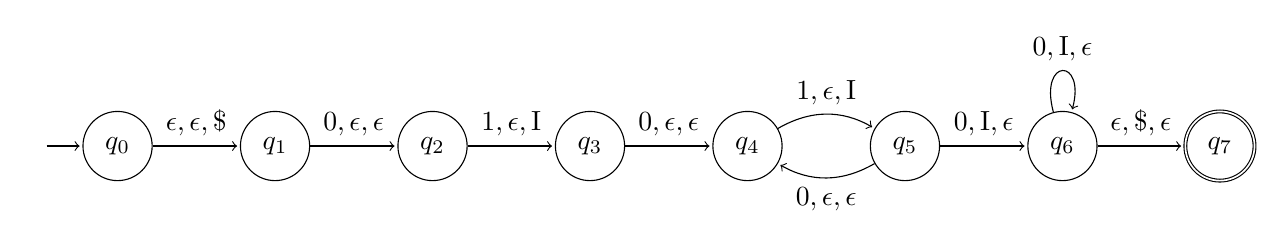
\begin{tikzpicture}[shorten >=1pt, node distance=2cm, on grid, auto]
        \node[state, initial, initial text=] (q0)   {$q_0$};
        \node[state] (q1) [right=of q0] {$q_1$};
        \node[state] (q2) [right=of q1] {$q_2$};
        \node[state] (q3) [right=of q2] {$q_3$};
        \node[state] (q4) [right=of q3] {$q_4$};
        \node[state] (q5) [right=of q4] {$q_5$};
        \node[state] (q6) [right=of q5] {$q_6$};
        \node[state, accepting] (q7) [right=of q6] {$q_7$};




        
        \path[->]
        (q0) edge  node {$\epsilon, \epsilon, \$$} (q1)
        (q1) edge node {$0, \epsilon, \epsilon$} (q2)
        (q2) edge node {$1,\epsilon, \text{I}$} (q3)
        (q3) edge node {$0,\epsilon, \epsilon$} (q4)
        (q4) edge [bend left] node {$1,\epsilon, \text{I}$} (q5)
        (q5) edge [bend left] node {$0,\epsilon, \epsilon$} (q4)
        (q5) edge node {$0, \text{I}, \epsilon$} (q6)
        (q6) edge [loop above] node {$0, \text{I}, \epsilon$} (q6)
        (q6) edge node {$\epsilon,\$, \epsilon$} (q7);
             
             
             
         
    \end{tikzpicture}
    \end{center}
    }

    Si scriva una grammatica context free equivalente all'automa a pila considerato.

    
    \addcontentsline{toc}{subsection}{Esercizio 46. (**)}\textcolor{orange}{\item \textbf{Esercizio 46. }}\textbf{(**)}\\ 
    Sia $L$ linguaggio c.f. su $\Sigma=\{0,1\}$, tale per cui 

    {
  \small
    \begin{center}
    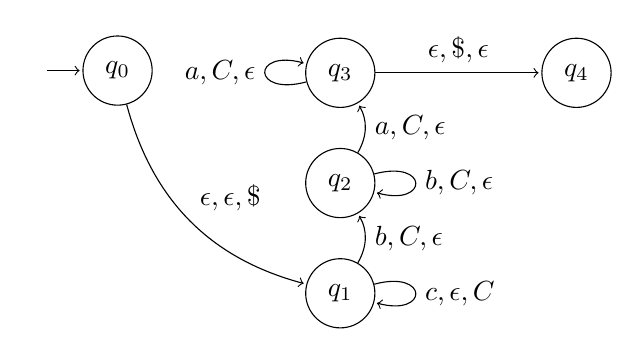
\begin{tikzpicture}[shorten >=1pt, node distance=2cm, on grid, auto]
        
        \node[state, initial, initial text=] (q0)   {$q_0$};
        \node[state] (q1) [below right=4of q0] {$q_1$};
        \node[state] (q2) [above=1.4of q1] {$q_2$};             
        \node[state] (q3) [above=1.4of q2] {$q_3$};     
        \node[state] (q4) [right=3of q3] {$q_4$};     


        \path[->]
        (q0) edge [bend right] node {$\epsilon, \epsilon,\$$} (q1)
        (q1) edge [loop right] node {$c,\epsilon,C$} (q1)
        (q1) edge [bend right, right] node {$b,C,\epsilon$} (q2)
        (q2) edge [bend right, right] node {$a,C,\epsilon$} (q3)
        (q2) edge [loop right] node {$b,C,\epsilon$} (q2)
        (q3) edge [loop left] node {$a,C,\epsilon$} (q3)
        (q3) edge node {$\epsilon,\$, \epsilon$} (q4);
        
    \end{tikzpicture}
    \end{center}
    }
    
    Si scriva una grammatica context free equivalente all'automa a pila considerato.
    
   
\end{itemize}
}
\vfill
\noindent\makebox[\linewidth]{\rule{\linewidth}{0.1pt}}
\end{document}
